\documentclass[a4paper,10.5pt]{report}

\usepackage[toc]{appendix}
\renewcommand{\appendixname}{Annexos}
\renewcommand{\appendixtocname}{Annexos}
\renewcommand{\appendixpagename}{Annexos}
\usepackage[catalan]{babel}
\usepackage{booktabs}
\usepackage{gensymb}
\usepackage{siunitx}
\usepackage[nottoc]{tocbibind}
\usepackage{listings}
\lstdefinestyle{mystyle}{
	language=Python,                 % Lenguaje del código
	frame=single,                    % Marco alrededor del código
	basicstyle=\ttfamily\footnotesize, % Fuente del código
	keywordstyle=\color{blue},       % Color para palabras clave (def, if, else...)
	commentstyle=\color{gray},       % Color para comentarios
	stringstyle=\color{teal},        % Color para strings
	numbers=left,                    % Numeración de líneas
	numberstyle=\tiny\color{gray},   % Estilo de los números de línea
	stepnumber=1,                     % Cada cuántas líneas numerar
	showspaces=false,                 % No mostrar espacios en blanco
	showstringspaces=false,            % No mostrar espacios en strings
	breaklines=true,                   % Romper líneas largas automáticamente
	tabsize=4,                         % Tamaño de tabulación
	captionpos=b,                      % Posición de la caption (arriba o abajo)
	morekeywords={self, as, in},       % Palabras clave adicionales
}
\lstset{style=mystyle} % Aplicar este estilo a todos los listados
\usepackage{tcolorbox}
\usepackage{parskip}
\usepackage{multirow}
\usepackage{graphicx}
\usepackage{booktabs}
\usepackage{caption}
\captionsetup{labelfont=bf}
\usepackage{hyperref}
\usepackage[arrowdel]{physics}
\usepackage[left=1.95cm, right=1.95cm, top=20mm, bottom=20mm]{geometry} 
\usepackage{fancyhdr}
\usepackage{braket}
\usepackage{amsmath, amssymb, amsfonts}
\usepackage{subcaption}
\usepackage{cancel}
\usepackage{float}
\usepackage{titling}
\usepackage{etoolbox}
\renewcommand{\labelenumi}{\textbf{\theenumi.}}
\usepackage{siunitx}
\sisetup{
	output-decimal-marker = {,},
	exponent-product = \cross
}

%Definim el següent entorn per tal de poder posar abstracts a cada capítol.
\newenvironment{chapterabstract}{
	\begin{center}
		\bfseries Abstract
	\end{center}
	\quotation
}{\endquotation}

\usepackage{titlesec}
\titlespacing*{\chapter}{0pt}{-30pt}{20pt}
\usepackage{tikz}

\usepackage{longtable}
\usepackage{adjustbox}

\titleformat{\chapter}[display]{\normalfont\LARGE\bfseries}{Part  \thechapter}{0pt}{\vspace{0.1cm}\Large\bfseries\raggedright}

\title{\textbf{\huge{Treball de Simulació. \\ \vspace{0.2cm} Termodinàmica i Mecànica Estadística}}}
\date{\today}

\begin{document}
	
	\begin{titlepage}
		\centering
		{\LARGE Termodinàmica i Mecànica Estadística \par}
		\vspace{3cm}
		{\Huge \textbf{Treball de Simulació}  \par}
		\vspace{4cm}
		{\Large Grau en Física \par}
		\vspace{1cm}
		{\Large 1549086: Bujones Umbert, Jun Shan\\ 1672980: González Barea, Eric\\1644841: Vilarrúbias Morral, Natàlia \par} 
		\vspace{0.5cm}
		\vspace{3cm}
		{\Large Maig 2026 \par}
		\vspace{2cm}
		
		\begin{figure}[h]
			\centering
			
\includegraphics[width=0.3\linewidth]{logo_uab}
			\label{fig:logouab}
		\end{figure}
		
		

	\end{titlepage}
	
	\pagenumbering{gobble}
	\newpage
	\thispagestyle{empty}

	\tableofcontents
	\newpage
	\pagenumbering{arabic}
	\setcounter{page}{1}
	
\chapter{Gas d'Esferes Dures}

\section{Introducció i fonament teòric}
En aquesta secció estudiarem un gas d'esferes dures. En aquest model, s'assumeix que el potencial d'interacció entre les diferents partícules del gas és tal que 
\begin{equation}
	\Phi(r) =
\begin{cases}
	 0 & \text{si } r>2r_0 \\
	 \infty & \text{si } r<2r_0
\end{cases}
\end{equation}
on $r$ és la distància entre dues partícules qualsevols i $r_0$ el seu radi atòmic. En particular, en aquesta part estudiarem l'He gas modelitzat segons aquest potencial. Treballarem en tot moment amb una simulació amb $N = 500$ àtoms d'He amb una massa de $m_{He} = 6,646 \cross 10^{-27}$ kg per àtom, a una temperatura de $T = 300$ K i compresos en una caixa cúbica de volum $V = 1$ m$^3$.

Els nostres objectius seran:
\begin{itemize}
	\item Estudiar com es veuen modificats els resultats de la simulació (la distribució de velocitats, entre d'altres), en funció del radi atòmic $r_0$ donat als àtoms d'He. A partir d'aquí seleccionar un radi òptim per a la resta de simulacions en funció dels resultats anteriors.
	\item Modificar la simulació original per tal que treballi sota la col·lectivitat canònica, utilitzant un termostat d'Andersen, tot analitzant la distribució d'energies que en resulta.
	\item Introduir a la simulació la presència d'un camp gravitatori en l'eix Z i veure com això afecta a la distribució de velocitats i les posicions en aquest mateix eix.
\end{itemize}

Recordem que, en equilibri tèrmic, la distribució de velocitats (o, més rigorosament, de celeritats) per un conjunt de partícules ve determinada per la distribució de Maxwell-Boltzmann
\begin{equation}
	\rho(v) = 4\pi v^2\left(\frac{m}{2\pi k_B T}\right)^{3/2}e^{-\frac{mv^2}{2k_B T}}.
\end{equation}

\textbf{COMENTAR EL TIPUS DE COL·LECTIVITAT. ÉS MICROCANÒNICA, AL LORO!}

\textbf{COMENTAR LES CONDICIONS INICIALS ($v_i$) DE LA SIMULACIÓ!}

\section{Estudi dels efectes del radi atòmic de l'He}
A la simulació original, es treballa amb $N=200$ àtoms i un radi atòmic de $r_0 = 0,03$ m, que és un valor molt més gran del radi atòmic conegut per a l'He, que és de 
\begin{equation*}
	r_{real} = 0,31 \text{ \AA} = 0,31\cross 10^{-10} \text{ m}.
\end{equation*}
La necessitat de treballar amb un radi atòmic tan gran està en el fet que la caixa cúbica usada té unes dimensions onze ordres de magnitud majors al radi real dels àtoms d'He
\begin{equation*}
	L \gg r_{real},
\end{equation*}
fet que, en treballar amb tan poca quantitat d'àtoms (originalment $N=200$), implica que les interaccions entre dues partícules són pràcticament inexistents, ja que la probabilitat de col·lisió és extremadament petita. Això fa que, en absència d'interaccions, el gas presenti un comportament pròxim a la idealitat. 

A continuació, analitzem, amb $N = 500$ àtoms, els següents casos: $r_0 = r_{real}$, $r_0 = 1,5$ m, $r_0 = 0,1$ m, $r = 0,01$ m i $r = 0,03$ m\footnote{Totes les simulacions es deixen funcionar durant un temps $t = 5$ minuts. En arribar a aquest $t$, les parem i analitzem els resultats obtinguts. Això ens permet determinar quina de les opcions és la que presenta un millor equilibri entre cost computacional i exactitud en els resultats.}. 

La distribució de velocitats que s'obté en usar el radi real $r_0 = r_{real}$ de l'heli és la que es mostra a la figura \ref{fig:1.1}. Tal i com podem veure, aquesta distribució de velocitats ens està indicant que no hi ha hagut, en essència, cap col·lisió, ja que pràcticament totes les partícules tenen exactament la mateixa velocitat que a l'inici. El resultat és, tal i com hem comentat abans, exactament el mateix que podríem esperar per un gas que no presenti interaccions intermoleculars, és a dir, un gas ideal (tot i que hem introduït un potencial d'interacció) i és degut al fet que el volum característic del sistema és excessivament major a l'ocupat per les partícules.

\begin{figure}[h]
	\centering
	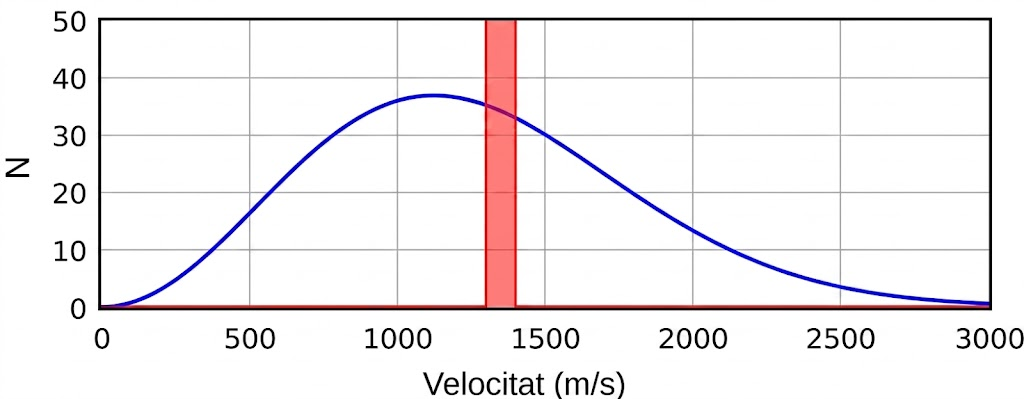
\includegraphics[width=0.5\linewidth]{dis_vels_r_real}
	\caption{Distribució de velocitats per $r_0 = r_{real}$ després de 5 minuts de simulació.}
	\label{fig:1.1}
\end{figure}

Si ara treballem amb un radi atòmic molt més gran, per exemple, de $r_0 = 1,5$ m, els resultats són els que es poden veure a la figura \ref{fig:1.2}. Podem veure com la distribució no s'adequa a una distribució de Maxwell-Boltzmann i, a més a més, en fer córrer la simulació, s'observa certa inestabilitat numèrica; fixem-nos en com, segons els resultats de la simulació, hi ha velocitats amb un $N<0$ associat, cosa que no és físicament plausible. Tot plegat és degut al fet que hem seleccionat un radi atòmic que és major que el volum de la pròpia caixa; en aquestes condicions les col·lisiones entre les molècules esdevenen contínues, erràtiques i representen una situació no física en què tenim una gran quantitat de partícules compresses en un volum més petit que les mateixes molècules. 

\begin{figure}[h]
	\centering
	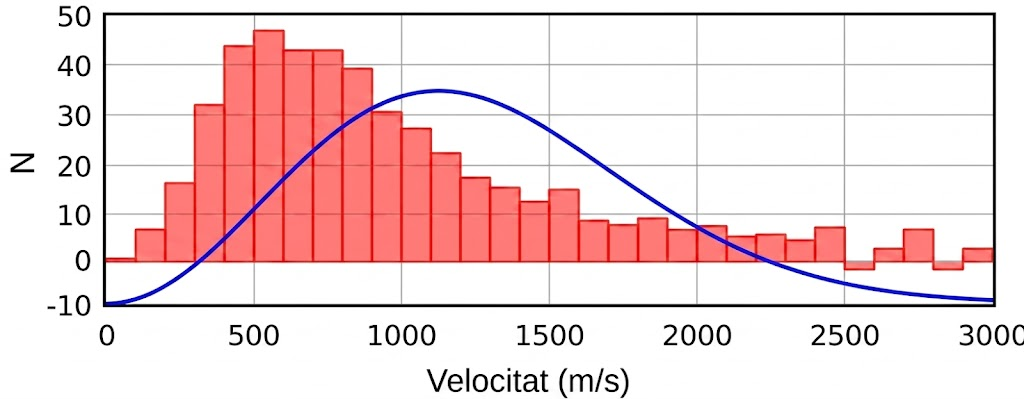
\includegraphics[width=0.5\linewidth]{dis_vels_r_1.5}
	\caption{Distribució de velocitats per $r_0 = 1,5$ m després de 5 minuts de simulació.}
	\label{fig:1.2}
\end{figure}

Si ara treballem amb $r_0 = 0,1$ m, obtenim els resultats de la figura \ref{fig:1.3}. Tot i que ara la distribució de velocitats és més similar a una distribució de Maxwell-Boltzmann que en els casos anteriors, encara podem veure una certa desviació respecte del comportament esperat. Això és degut, fonamentalment, a que, tot i que el radi de les partícules és suficientment gran com per garantir que les col·lisions es produeixin ràpidament, és encara excessivament gran comparat amb la longitud característica de la caixa, fet que provoca que, en tenir una quantitat tan gran de partícules de radi només un ordre de magnitud menor al volum de la caixa, moltes quedin sol·lapades unes amb altres, fent que hi hagi col·lisions contínues, és a dir, contacte no interromput entre dues partícules. Tot plegat fa que els resultats es desviïn respecte del que caldria esperar.

\begin{figure}[H]
	\centering
	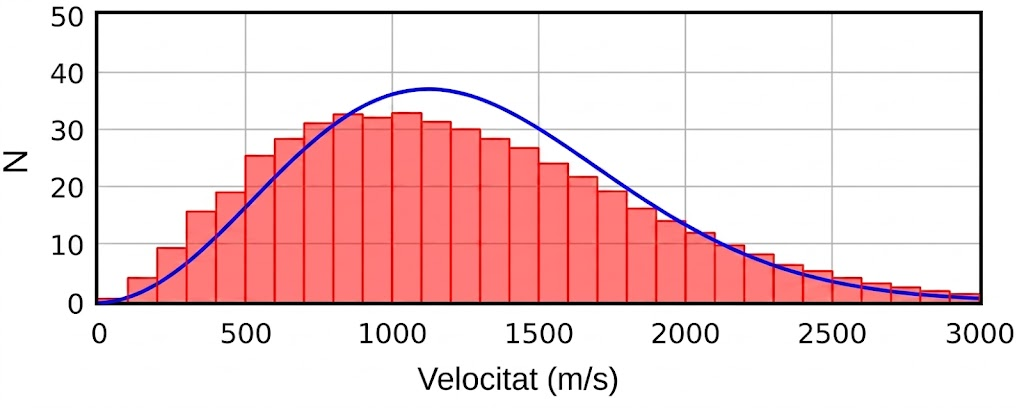
\includegraphics[width=0.5\linewidth]{dis_vels_r_0.1}
	\caption{Distribució de velocitats per $r_0 = 0,1$ m després de 5 minuts de simulació.}
	\label{fig:1.3}
\end{figure}

Si escollim $r_0 = 0,01$ m, s'obtenen els resultats de la \ref{fig:1.4}. Podem veure com la distribució de velocitats s'assembla molt més a la predita teòricament, però encara hi ha certes discrepàncies. Els àtoms d'He encara són massa petits com per garantir que, amb només 5 minuts de simulació, s'assoleixi l'equilibri tèrmic (i, per tant, la distribució obtinguda s'adapti perfectament a la de Maxwell-Boltzmann).

\begin{figure}[h]
	\centering
	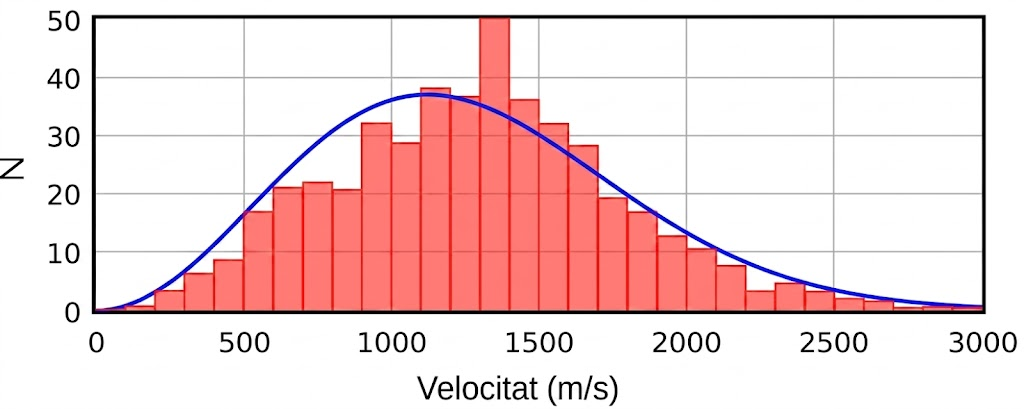
\includegraphics[width=0.5\linewidth]{dis_vels_r_0.01}
	\caption{Distribució de velocitats per $r_0 = 0,01$ m després de 5 minuts de simulació.}
	\label{fig:1.4}
\end{figure}

Si escollim $r_0 = 0,03$ m, s'obtenen els resultats de la figura \ref{fig:1.5}. Veiem com ara sí que obtenim uns resultats compatibles amb la predicció teòrica. L'única diferència important és que tenim encara més partícules de les esperades amb la velocitat inicial, però aquest valor no és massa discrepant. De fet, si augmentem el temps de simulació a 20 minuts, tal i com es pot veure a la figura \ref{fig:1.5b}, els resultats són perfectament compatibles amb la distribució de Maxwell Boltzmann.

\begin{figure}[H]
	\centering
	\begin{subfigure}{0.48\linewidth}
		\centering
		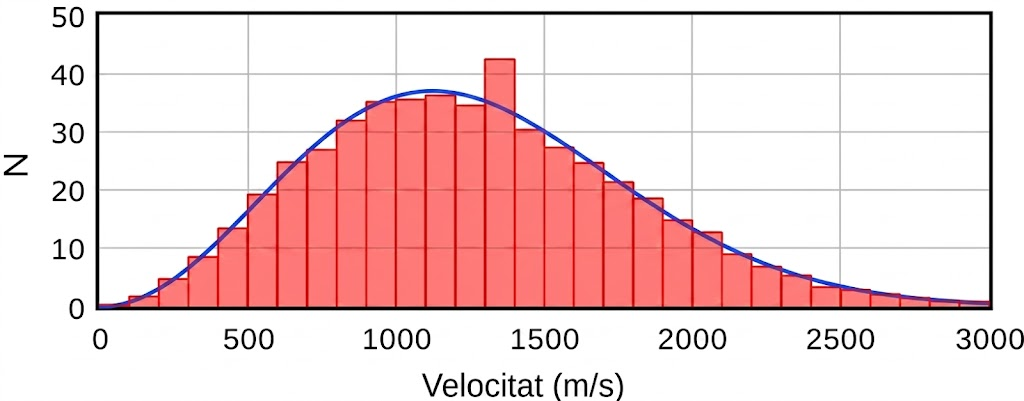
\includegraphics[width=\linewidth]{dis_vels_r_0.03}
		\caption{Després de 5 minuts de simulació.}
		\label{fig:1.5a}
	\end{subfigure}
	\hfill
	\begin{subfigure}{0.48\linewidth}
		\centering
		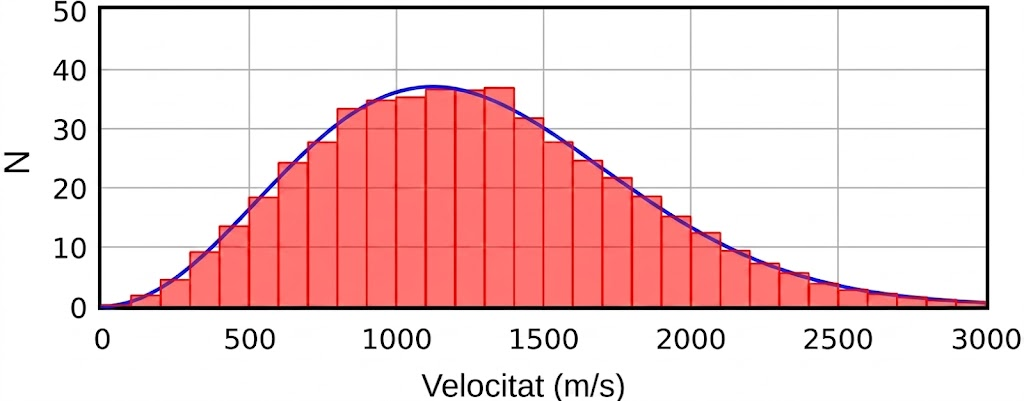
\includegraphics[width=\linewidth]{dis_vels_r_0.03_T=20min}
		\caption{Després de 20 minuts de simulació.}
		\label{fig:1.5b}
	\end{subfigure}
	\caption{Distribució de velocitats per $r_0 = 0{,}03$ m.}
	\label{fig:1.5}
\end{figure}

Els resultats obtinguts es troben resumits a la \ref{tab:1.1}. Calculem la proporció de volum total ocupat pel conjunt de partícules $p_{ocup.}$ simulades segons
\begin{equation}
	p_{ocup.} \equiv \frac{N\cdot V_{i}}{V} = \frac{4N\pi r_0^3}{3V}.
\end{equation}
Aquesta quantitat ens dóna una idea de com de saturada està la nostra caixa del gas d'esferes dures i, per tant, està relacionada amb la densitat d'aquest i la probabilitat de col·lisió (interacció) entre dues partícules del gas.

Per una banda, densitats altes implicaran probabilitats de col·lisió elevades, fent que s'arribi més ràpidament a la situació d'equilibri tèrmic i, per tant, a assolir una distribució de velocitats de Maxwell-Boltzmann; simultàniament, però, s'augmenta la probabilitat de que apareguin errors i inestabilitats en el càlcul numèric, associats a partícules que mantenen un contacte continu, entre d'altres. En casos extrems, en què $p_{ocup.} > 1$, els resultats no es corresponen amb una situació física.

Per altra banda, densitats baixes faran que els errors i les inestabilitats del mètode numèric disminueixin, però a costa de disminuir progressivament la probabilitat de col·lisió i, per tant, d'interacció, entre els constituents del gas. Això resultarà en la necessitat de temps de simulació més elevats per garantir que les interaccions intermoleculars són suficients com per assolir l'equilibri tèrmic i, per tant, que la distribució de velocitats s'adeqüi a la predita teòricament. En casos extrems, en què $p_{ocup.} \ll 1$, pràcticament no hi ha interacció entre partícules i, per tant, tots els àtoms d'He romanen amb la mateixa velocitat que al principi de la simulació.

\begin{table}[h]
	\centering
	\caption{Taula amb els radis usats per l'àtom d'He i les corresponents ocupacions del gas respecte del volum total del recipient.}
	\begin{tabular}{l c}
		\toprule
		$r_0$ (m) & $p_{ocup.}$ \\
		\midrule
		$0{,}34\cross10^{-10}$ & $6{,}24\cross10^{-29}$ \\
		$1{,}50$   & $7{,}07\cross10^3$ \\
		$0{,}10$   & $2{,}09$ \\
		$0{,}010$  & $2{,}09\cross10^{-3}$ \\
		$0{,}030$  & $5{,}65\cross10^{-2}$ \\ 
		\bottomrule
	\end{tabular}
	\label{tab:1.1}
\end{table}
 
\textbf{VALORAR SI VAL LA PENA POSAR $r = 0,04$. MILLORS RESULTATS EN MENYS TEMPS.}

\section{Col·lectivitat canònica i anàlisi de la distribució d'energies}

\section{Addició d'un potencial gravitatori} 


\chapter{Fluid de Lennard-Jones}

\section{Introducció i fonament teòric}

\section{Estudi d'estats estacionaris}

\section{Anàlisi del coeficient de compressibilitat isoterma}

	
\chapter{Creació d'una simulació pròpia}

\section{Introducció i fonament teòric}

\section{Modelització i implementació de la regla de Metropolis}

\section{Anàlisi dels resultats}

\subsection{Ocupació mitjana en funció de la temperatura}

\subsection{Estudi de les fluctuacions en l'energia}

\begin{thebibliography}{99}
\bibitem{ref1}
\textit{Col·lecció de problemes de l'assignatura Termodinàmica i Mecànica Estadística}.

\end{thebibliography}

\end{document}